\chapter{Overview of Pattern Recognition Techniques}

In this chapter, we will discuss the mathematical foundations of the patern recognition methods that will be used to predict 
scores. There are two approaches to this. The first is to use already built packages for both a given programming language and simply
feed data into it and present the results. The second method is to build them from scratch. The disadvantage to doing this is naturally 
that it is more time consuming. However, it does allow for more control over how our models work, and will allow us to understand our results
better, than if we had used a proprietary model. This isn't to say that the code written for these models won't utilise packages for doing things
like linear algebra calculations, but we wont simply import a neural network package and have results within 5 lines of code. \\

%Explain which langauges were chosen for each method and why


\section{Neural Networks}

\subsection{A Brief Introduction to Neural Networks}
Neural networks (NNs) have been the subject to a lot of hype in recent years. They are a machine learning method that is being applied to many problems
in all sorts of fields.  %some references here please 
The network will be trained on runrate data, so for each game we have calculated the evolution of the runrate,
and then we have the overall score for that game in the final column of the matrix. An example of a network can be seen in \ref{nnexample1}. The first layer is the 
input layer, and the last layer gives the predictions. The middle layers are hidden and where the work of the network is done. \\

Let's look at what a NN actually looks like. The below is an example of a network with just one hidden layer.

\begin{figure}
    \centering
    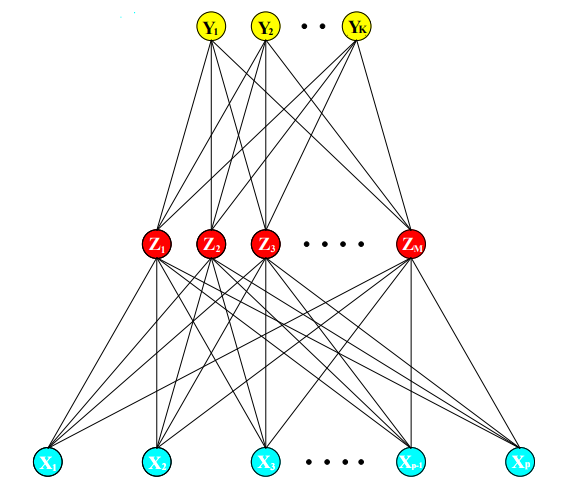
\includegraphics[scale=0.5]{figures/nn.png}
    \caption{Example of a single hidden layer neural network, as in \cite{sprbk}}
    \label{nnexample1}
\end{figure}

We see there are $p$ input nodes at the bottom, M nodes in the hidden layer, and K output layers. The lines between the layers are given a ``weight''
and a ``bias''. These properties will be discussed in more detail shortly. The number of hidden layers to be used will be the subject of experimentation. In order to find try this out, we will have to randomly
split the matrix into a training matrix and a testing matrix. We can then evaluate the network by trying to predict values from the testing set and seeing
how well it does. This will then lead to us refining the number of hidden layers as appropriate. \\

One area of the world where neural networks are being applied to value prediction is in the stock market. Naturally if one can predict how the value of a stock
will change over some time period, then one can protect themself from a bad investment, or profit heavily from a good one. We will use similar
methods here for building our neural network.  In \cite{nnstock}, the authors twest two different Neural Netowrks, and find that using a ``Multi-Layer Feed Forward Nerual Network''
is the better choice for predicting how stock values will change. With these motivations in mind, we can begin to construct the networks.

\subsection{Builiding The Network}
%Rewrite this bit
Our input layer will have 50 nodes, one for the runrate at the end of each over. We will begin with 5 hidden layers, although this is subject to change. The output layer
will of course only have one node, the value of which will predict the score of the game. 

We begin by looking at a single node. The proper name for each node is ``perceptron''. Each perceptron takes in the values of a vector, and an extra ``+1'' intercept term. The perceptron then outputs a valye h given by \ref{percepout}:

\begin{equation}
    \label{percepout}
    h_{W,b}(x) = f(\textbf{W}^Tx) = f(\sum_{i=1}^KW_ix_i+b).
\end{equation}

Here, $K \in \mathbb{N}$ is the number of elements in the vector, and $f:\mathbb{R} \rightarrow \mathbb{R}$ is called the activation function. There is a bit of choice in which activation function to use.
The two common choices are:

\begin{align}
    f(z) &= \frac{1}{1+exp(-z)} \\
    f(z) &= tanh(z)
\end{align}

The comparrison of these two functions can be seen in \ref{actfig}.

\begin{figure}[h]
    \centering
    \label{actfig}
    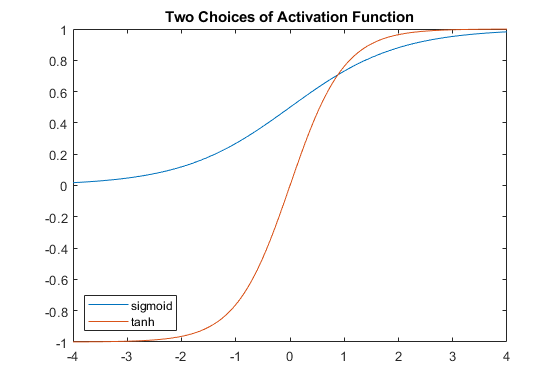
\includegraphics[scale=0.5]{figures/actfuncs.png}
    \caption{Graph showing the shape of different activation functions.}
\end{figure}

We will be using (5.2) as our activation but will return to the activation function shortly. For now, lets look at the network we're going to use.
The initial neural network that we're building. The code for this activation can be seen in \ref{pyact}, note we have included the derivative of this function too, which will be important later.

\begin{figure} %MAKE SURE THESE ARE THE RIGHT LINES OF CODE!!
    \lstinputlisting[language=Python, firstline=14,lastline=18]{../code/net.py}
    \caption{Python code for the activation function}
    \label{pyact}
\end{figure}

%Put a picture of the network here when you make it

We begin with getting from the input layer, denoted $L_0$. Each node in $L_0$ takes a value $a^{(0)_i}$ for $i \in \{1,2,\ldots,50\}$. We use $\textbf{a}^{(0)}$ to denote the vector
containing these values. For every node in $L_0$, we have 25 connections coming away, one going to each of the nodes in $L_1$. 25 was an arbitraty choice for the size of $L_1$, and is
subject to change based on results from initial testing. So that means we have $50 \times 25 = 1250$ weights for just the first layer alone. Some linear algebra is to be done here to get 
values for the vector $\textbf{a}^{(1)}$. We use $w_ij$ to denote the weight from node j in one layer to node i in the prior layer. We can then construct a matrix containing the weights
between $L_0$ and $L_1$, which we denote $W^{(1)}$. This matrix is given by \ref{weights1}.

\begin{equation}
    W^{(1)} =
    \left[ {\begin{array}{cccc}
      w_{1,1} & w_{1,2} & \cdots & a_{1,50}\\
      w_{2,1} & w_{2,2} & \cdots & a_{2n}\\
      \vdots & \vdots & \ddots & \vdots\\
      w_{25,1} & a_{25,2} & \cdots & a_{25,50}\\
    \end{array} } \right]
    \label{weights1}
\end{equation}

Using \ref{weights1}, and combining with $a^{(0)}$, we can get the following:

\begin{align}
    A^{(1)} &= \left[ {\begin{array}{cccc}
        w_{1,1} & w_{1,2} & \cdots & a_{1,50}\\
        w_{2,1} & w_{2,2} & \cdots & a_{2n}\\
        \vdots & \vdots & \ddots & \vdots\\
        w_{25,1} & a_{25,2} & \cdots & a_{25,50}\\
      \end{array} } \right] \times \left[ \begin{array}{c}
          a^{(0)}_1 \\
          a^{(0)}_2 \\
          \vdots \\
          a^{(0)}_{50} \\
      \end{array} \right] + \left[ \begin{array}{c}
        b^{(0)}_1 \\
        b^{(0)}_2 \\
        \vdots \\
        b^{(0)}_{25} \\
        \end{array} \right] \\
      &= W^{(1)}\textbf{a}^{0} + \textbf{b}^1
\end{align}

Where $\textbf{b}^1$ is the vector containing the biases for each node.  At this point, we are incredibly close to having values for $\textbf{a}^{(1)}$. The last thing to do
is apply the activation function. The above has resulted in a $25\times 1$ vector, we use the notation $f(A^{(1)})$ to denote applying the activation function to each 
element in the vector $A^{(1)}$. Putting this all together, we have the following equation:

\begin{equation}
    \textbf{a}^{(1)} = f(W^{(1)}\textbf{a}^{(0)} + \textbf{b}^{1})
\end{equation}

Which gives us values for all the nodes in the first hidden layer. This process is then repeated for all the the remaining layers in the network. Implementing this in Python 
is not too difficult, and the code can be seen in \ref{pyActVals}. The only function that can be seen here with no code is $\textit{is\_Valid()}$, which just checks that all the 
constituents are of the right dimensions. If this returns false, then it wont let the calculations go ahead. 

\begin{figure}[h]%AGAIN, MAKE SURE THESE ARE THE RIGHT LINES OF CODE!!
    \lstinputlisting[language=Python, firstline=29,lastline=45]{../code/net.py}
    \caption{Python code for giving activation values to the next layer}
    \label{pyActVals}
\end{figure}


This process is then repeated for each layer, creating a diffferent weights and bias matrix going between each layer in the network. These matrices are naturally of different sizes, but the principle is exactly the same.
When we start the training process for this network, we will only have random variables for the weights and biases. To gain better values that can predict accurate results in the future,
we need to train the network by feeding it feature vectors and their associated outputs. \\

To allow the netowrk to be trained, we first must define a ``cost function''. The way we do this is to input a vector to the input layer, let the network produce a result, say $y'$, which
initially will be hooribly wrong, and square the difference between this and the true value $y$ for that particluar training vector. Put more precisely,
let \textbf{X} be a feature vector containing 50 elements, and $y$ the corresponding output. Then define the cost function, $C(X,y) := (y'-y)^2$. The lower the value of $C(X,y)$, the 
better the network has done at predicting. The average value of $C(X,y)$ for each X and y in our training set, is then a good measure of the network's performance. \\

The cost function is at the heart of how these networks ``learn''. All we're doing is minimising a cost function, to give matrices of weights and biases that
produce the best output. The algorithm for minimising this cost function is called ``gradient descent'' \cite{cauchy}. Suppose we take every single weight and bias of our network,
and turn it into a giant column vector. 

\begin{example}
    In this first example, we initialise four random weights matrices, four bias vectors, and we run through the process outlined above. We know going into this that 
    the cost is going to be high. Initialising the weights as random values $w_{ij} \in [-1000,1000]$, we get an initial cost function for our full dataset of a huge
    3098.4. 
\end{example}

\subsection{Gradient-Descent and Backpropogation}

We discussed in section \ref{mse} the need to use a MSE loss function based on our data. Let us now define this function, as in \cite{huber}.

\begin{definition}
    Let N be the number of datapoints, $y_i'$ be the prediceted value from the $i^{th}$ datapoint, and $y_i$ be the true value. Then for the input vector X, and a parameter $\theta$,
    define the \textbf{Mean Square Error} by
    \begin{equation}
        E(X,\theta) = \frac{1}{2N}\sum^N_{i=1}(y_i'-y_i)^2
    \end{equation}
\end{definition}

The method of \textit{Gradient Descent} necessitates calculating the gradient of $E(X,\theta)$ with respect to weights and biases in each layer. The idea is to find a local minimum, as this will
give a set of weights and biases for which the error is lowest, and such that the network is giving well approximated results. Define a \textit{learning rate} $\alpha$, and incorperate the set of weights
and biases into the parameter $\theta$. Then we update the weights and biases each iteration t via the relationship \ref{graddesc}

\begin{equation}
    \label{graddesc}
    \theta^{t+1} = \theta^t - \alpha\frac{\partial E(X,\theta)}{\partial \theta}.
\end{equation}

With this in mind, we can now start to go through the Backpropogation process. Firstly, we need to calculate the partial differential of E with respect to a given weight $w_{ij}$. This calculation is given as follows:

\begin{align}
    \frac{\partial E(X,\theta)}{\partial w_{ij}^k} &= \frac{1}{2N}\sum_{d=1}^N\frac{\partial (y'_d-y_d)^2}{\partial w_{ij}^k} \\
                                                   &= \frac{1}{N}\sum^N_{d=1} \frac{\partial E_d(X,\theta)}{\partial w_{ij}^k}
\end{align}

In the above, we have $E_d = \frac{1}{2}(y'_d-y_d)^2$.  We must emply the chain rule to calculate the partial derivavtive of $E_d$ with respect to an individual weight. 
Let $a_j^k$ be the activation value of node j in layer k before it is put through the activation function. Then we have

\begin{equation}
    \label{errorchain}
    \frac{\partial E}{\partial w_{ij}^k} = \frac{\partial E}{\partial a_j^k}\frac{\partial a_j^k}{\partial w_{ij}^k}
\end{equation}

In \ref{errorchain}, the first derivative on the righthand side, is known as the \textit{error}, often denoted as $\delta_j^k$. The second derivative on that side
is the \textit{output} of node i in layer $k-1$, denoted $o_i^{k-1}$. So we can simplify \ref{errorchain} to be written as

\begin{equation}
    \frac{\partial E}{\partial w_{ij}^k} = \delta^k_jo_i^{k-1}.
\end{equation}

The aim of backpropogation is to $\delta^m_1$, where m denotes the final layer. We can express $E_d$ in terms of $a_1^m$ as follows:

\begin{equation}
    E_d = \frac{1}{2} (f(a_1^m)-y_d)^2.
\end{equation}

Where $f$ is the activation function. We have:

\begin{equation}
    \delta_1^m = (y'-y)f'(a_1^m).
\end{equation}

So in the final layer, we have:

\begin{align}
    \frac{\partial E_d}{\partial w_{i1}^m} &= \delta_1^mo_i^{m-1} \\
                                           &= (y_d'-y_d)f'(a_1^m)o_i^{m-1}.
\end{align}

The above is all well and good for the final layer, but we now must consider the hidden layers. We will consider the general case here, and then plug in the relevant
numbers for our model when it comes to the implementation later on. For a layer k such that $1 \leq k < m$, the error term $\delta^k_j$ is given by:

\begin{align}
    \delta_j^k &= \frac{\partial E_d}{\partial a_j^k} \\
               &= \sum_{l=1}^{r^{k+1}} \frac{\partial E_d}{\partial a_l^{k+1}}\frac{\partial a_l^{k+1}}{\partial a_j^k}.
\end{align}

In the above, $r^{k+1}$ is the number of nodes in the next layer, and $ l = 1,2,\ldots,r^{k+1}$. Since we can write $\delta_l^{k+1} = \frac{\partial E_d}{\partial a_l^{k+1}}$, the above can be written
as 

\begin{equation}
    \label{deltajk}
    \delta_j^k = \sum_{l=1}^{r^{k+1}}\delta_l^{k+1}\frac{\partial a_l^{k+1}}{\partial a_j^k}.
\end{equation}

Since the activation of a layer in one node is the sum of weights and avtications in the prior layer, we write:

\begin{equation}
    a_l^{k+1} = \sum^{r^k}_{j=1} w_{jl}^{k+1}f(a_j^k).
\end{equation}

Therefore,

\begin{equation}
    \frac{\partial a_l^{k+1}}{\partial a_j^k} = w_{jl}^{k+1}f'(a_j^k).
\end{equation}

Plugging the above in \ref{deltajk}, we obtain the following:

\begin{equation}
    \label{backpropform}
    \delta_j^k = f'(a_j^k)\sum^{r^{k+1}_{l=1}}w_{jl}^{k+1}\delta_l^{k+1}.
\end{equation}

The equation \ref{backpropform} is known as the \textit{Backpropogation formula}. The final step is to calculate, $\frac{\partial E_d}{\partial w_{ij}^k}$, which is given by:

\begin{align}
        \frac{\partial E}{\partial w_{ij}^k} &= \delta^k_jo_i^{k-1} \\
        &=f'(a_j^k)o^{k-1}_i \sum^{r^{k+1}}_{l=1}w_{jl}^{k+1}\delta_l^{k+1}.
\end{align}
